
\documentclass[usenames,dvipsnames,aspectratio=169,11pt, envcountsect, handout]{beamer}
%handout,
%aspectratio=43

\usepackage{Others/prespreamble}
\usepackage{natbib}
\definecolor{blue}{rgb}{0.19, 0.55, 0.91}
\linespread{1}
\usepackage{mathrsfs}

% small bibliography
\let\oldthebibliography=\thebibliography
\renewcommand{\thebibliography}[1]{
    \oldthebibliography{#1}
    \setlength{\itemsep}{2pt}
    \tiny
}

\begin{document}

\section{Introduction}

\begin{frame}[noframenumbering,plain]
	\maketitle
	%\begin{figure}[H]
	%\centering
	%\includegraphics[scale=0.4]{Other/Figures/erc.png}
	%\end{figure}

	%\footnotesize{Funding from the European Research Council (ERC) under the European Unions Horizon 2020 research and innovation programme (grant agreement No. 789111 - ERC EvolvingEconomics) is gratefully acknowledged}
\end{frame}
%\frame{\titlepage}

\begin{frame}\frametitle{Motivation}

	Individuals derive pleasure or pain from having specific beliefs.

	\vfill

	Consequently, they avoid or distort information:

	\vfill

	\begin{wideitemize}
		\item investors overreact to good news \citep{danielOverconfidentInvestorsPredictable2015};
		\item donors are uninformed about their impact \citep{niehausTheoryGoodIntentions2014};
		\item medical patients avoid testing \citep{golmanInformationAvoidance2017}.
	\end{wideitemize}

	\vfill

	Economists need models aligned with these phenomena for prediction and policy.

\end{frame}

\begin{frame}\frametitle{Belief-dependent preferences}

	Proposal: Belief-dependent preferences \citep{benabou2016mindful,koszegiUtilityAnticipationPersonal2010}.

	\vfill

	Three drawbacks:

	\vfill

	\begin{wideitemize}
		\item object of choice unobservable, such as beliefs, probability to forget;
		\item no identification, many pairs of beliefs and preferences are choice equivalent;
		\item BDP and non-Bayesian updating are disjoint assumptions.
	\end{wideitemize}

	\vfill \pause

	\textbf{This paper}:
	\vfill
	\begin{wideitemize}
		\item propose novel observable choice data allowing identification (if and only if);
		\item BDP imply a specific form of non-Bayesian updating.
	\end{wideitemize}

\end{frame}

\begin{frame}\frametitle{This Paper}

	Preferences depend on the individual's posterior beliefs.

	\vfill

	The individual distorts beliefs away from Bayesian updating to increase her welfare.

	\vfill

	She then acts according to her distorted beliefs.

	\vfill

	Ex-ante, she anticipates such belief and choice distortion \citep{cobb-clarkPredictivePowerSelfcontrol2022}.

	\vfill \pause

	\textbf{Main result}: axiomatic characterisation of BDP preferences and updating rules.

\end{frame}

\begin{frame}{Illustrative Example}

	An investor decides whether to check the balance in her portfolio.

	\vfill

	If she does, she observes price \( p \) and can invest \( \left( i_{p} \right) \) or withdraw \( \left( w_p \right) \). \pause

	\vfill

	\begin{table}[H]
		\centering
		\begin{minipage}{0.29\textwidth}

		\end{minipage}\hspace{0.3cm} % Adjust the horizontal space between the tables and the symbol
		% Symbol goes here
		\begin{minipage}{0.29\textwidth}
			\centering
			\begin{tabular}{c | c}
				\multicolumn{2}{c}{\textbf{Check}}                                     \\
				State                & Menus                                           \\
				\hline
				{\color{blue}Good}   & \multirow{2}{*}{{\color{blue}\( i_{p}, w_p \)}} \\
				{\color{blue}Normal} &                                                 \\
				Bad                  & \(  i_{q}, w_q \)                               \\
			\end{tabular}
			\vspace{0.5cm} % Adjust vertical space between tables and caption
		\end{minipage}\hspace{0.3cm} % Adjust the horizontal space between the tables and the symbol
		% Symbol goes here
		\begin{minipage}{0.29\textwidth}

		\end{minipage}
		%\caption{Commitment under positive prior belief to avoid excessive investment.} % Add your caption here
		%\label{tab:commitment}
	\end{table} \pause

	\vfill

	Upon observing price \( p \), she infers the state of the market is not bad.

	\vfill

	When she sees price \( q \), she knows the state of the market is bad.

\end{frame}

\begin{frame}[noframenumbering]{Illustrative Example}

	Before checking, she anticipates to overweight evidence and invest too much.

	\vfill

	However, she might want to check anyway to obtain pleasant information. \pause

	\vfill

	\begin{table}[H]
		\centering
		\begin{minipage}{0.29\textwidth}

		\end{minipage}\hspace{0.3cm} % Adjust the horizontal space between the tables and the symbol
		% Symbol goes here
		\begin{minipage}{0.29\textwidth}
			\centering
			\begin{tabular}{c | c}
				\multicolumn{2}{c}{\textbf{Check}}                                     \\
				State                & Menus                                           \\
				\hline
				{\color{blue}Good}   & \multirow{2}{*}{{\color{blue}\( i_{p}, w_p \)}} \\
				{\color{blue}Normal} &                                                 \\
				Bad                  & \(  i_{q}, w_q \)                               \\
			\end{tabular}
			\vspace{0.5cm} % Adjust vertical space between tables and caption
		\end{minipage}\hspace{0.5cm} % Adjust the horizontal space between the tables and the symbol
		\( \succ \)
		\begin{minipage}{0.29\textwidth}
			\centering
			\begin{tabular}{c | c}
				\multicolumn{2}{c}{\textbf{Not Check}} \\
				State  & Menus                         \\
				\hline
				Good   & \multirow{3}{*}{ \( 0 \)}     \\
				Normal &                               \\
				Bad    &                               \\
			\end{tabular}
			\vspace{0.5cm} % Adjust vertical space between tables and caption
		\end{minipage}
		\caption{Excessive investment.} % Add your caption here
		\label{tab:excess}
	\end{table} \pause

	\vfill

	\textbf{Trade-off}: not receiving information vs acting under a distorted belief.

\end{frame}

\begin{frame}[noframenumbering]{Illustrative Example}

	She might also prefer not to check because she expects unpleasant information.

	\vfill

	\begin{table}[H]
		\centering
		\begin{minipage}{0.29\textwidth}

		\end{minipage}\hspace{0.3cm} % Adjust the horizontal space between the tables and the symbol
		% Symbol goes here
		\begin{minipage}{0.29\textwidth}
			\centering
			\begin{tabular}{c | c}
				\multicolumn{2}{c}{\textbf{Check}}                                     \\
				State                & Menus                                           \\
				\hline
				{\color{blue}Good}   & \multirow{2}{*}{{\color{blue}\( i_{p}, w_p \)}} \\
				{\color{blue}Normal} &                                                 \\
				Bad                  & \(  i_{q}, w_q \)                               \\
			\end{tabular}
			\vspace{0.5cm} % Adjust vertical space between tables and caption
		\end{minipage}\hspace{0.5cm} % Adjust the horizontal space between the tables and the symbol
		\( \prec  \)
		\begin{minipage}{0.29\textwidth}
			\centering
			\begin{tabular}{c | c}
				\multicolumn{2}{c}{\textbf{Not Check}} \\
				State  & Menus                         \\
				\hline
				Good   & \multirow{3}{*}{ \( 0 \)}     \\
				Normal &                               \\
				Bad    &                               \\
			\end{tabular}
			\vspace{0.5cm} % Adjust vertical space between tables and caption
		\end{minipage}
		\caption{Information avoidance under negative prior beliefs, "ostrich effect".} % Add your caption here
		\label{tab:oistrich}
	\end{table} \pause

	Both excessive trading and the ostrich effect constitute empirical puzzles in finance \citep{danielOverconfidentInvestorsPredictable2015,golmanInformationAvoidance2017}.

\end{frame}

\begin{frame}[noframenumbering]{Illustrative Example}

	\textbf{Solution}: delegate to a financial advisor, allowing her to commit not to invest. \pause

	\vfill

	\begin{table}[H]
		\centering
		\begin{minipage}{0.29\textwidth}
			\centering
			\begin{tabular}{c | c}
				\multicolumn{2}{c}{\textbf{Delegate}}                           \\
				State                & Menus                                    \\
				\hline
				{\color{blue}Good}   & \multirow{2}{*}{{\color{blue}\( w_p \)}} \\
				{\color{blue}Normal} &                                          \\
				Bad                  & \( w_q \)                                \\
			\end{tabular}
			\vspace{0.5cm} % Adjust vertical space between tables and caption
		\end{minipage}\hspace{0.5cm} % Adjust the horizontal space between the tables and the symbol
		% Symbol goes here
		\begin{minipage}{0.29\textwidth}
			\centering
			\begin{tabular}{c | c}
				\multicolumn{2}{c}{\textbf{Check}}                                     \\
				State                & Menus                                           \\
				\hline
				{\color{blue}Good}   & \multirow{2}{*}{{\color{blue}\( i_{p}, w_p \)}} \\
				{\color{blue}Normal} &                                                 \\
				Bad                  & \(  i_{q}, w_q \)                               \\
			\end{tabular}
			\vspace{0.5cm} % Adjust vertical space between tables and caption
		\end{minipage}\hspace{0.5cm} % Adjust the horizontal space between the tables and the symbol
		% Symbol goes here
		\begin{minipage}{0.29\textwidth}
			\centering
			\begin{tabular}{c | c}
				\multicolumn{2}{c}{\textbf{Not Check}} \\
				State  & Menus                         \\
				\hline
				Good   & \multirow{3}{*}{ \( 0 \)}     \\
				Normal &                               \\
				Bad    &                               \\
			\end{tabular}
			\vspace{0.5cm} % Adjust vertical space between tables and caption
		\end{minipage}
		%\caption{Commitment under positive prior belief to avoid excessive investment.} % Add your caption here
		%\label{tab:commitment}
	\end{table}

\end{frame}

\begin{frame}[noframenumbering]{Illustrative Example}

	Commitment allows her to obtain information without being tempted to overinvest.

	\vfill

	\begin{table}[H]
		\centering
		\begin{minipage}{0.29\textwidth}
			\centering
			\begin{tabular}{c | c}
				\multicolumn{2}{c}{\textbf{Delegate}}                           \\
				State                & Menus                                    \\
				\hline
				{\color{blue}Good}   & \multirow{2}{*}{{\color{blue}\( w_p \)}} \\
				{\color{blue}Normal} &                                          \\
				Bad                  & \( w_q \)                                \\
			\end{tabular}
			\vspace{0.5cm} % Adjust vertical space between tables and caption
		\end{minipage}\hspace{0.3cm} % Adjust the horizontal space between the tables and the symbol
		\( \succ \) % Symbol goes here
		\begin{minipage}{0.29\textwidth}
			\centering
			\begin{tabular}{c | c}
				\multicolumn{2}{c}{\textbf{Check}}                                     \\
				State                & Menus                                           \\
				\hline
				{\color{blue}Good}   & \multirow{2}{*}{{\color{blue}\( i_{p}, w_p \)}} \\
				{\color{blue}Normal} &                                                 \\
				Bad                  & \(  i_{q}, w_q \)                               \\
			\end{tabular}
			\vspace{0.5cm} % Adjust vertical space between tables and caption
		\end{minipage}\hspace{0.3cm} % Adjust the horizontal space between the tables and the symbol
		\( \succ \) % Symbol goes here
		\begin{minipage}{0.29\textwidth}
			\centering
			\begin{tabular}{c | c}
				\multicolumn{2}{c}{\textbf{Not Check}} \\
				State  & Menus                         \\
				\hline
				Good   & \multirow{3}{*}{ \( 0 \)}     \\
				Normal &                               \\
				Bad    &                               \\
			\end{tabular}
			\vspace{0.5cm} % Adjust vertical space between tables and caption
		\end{minipage}
		\caption{Commitment under positive prior belief to avoid excessive investment.} % Add your caption here
		\label{tab:commitment}
	\end{table}

	\vfill

	Commitment might be welfare enhancing under belief-dependent preferences.

\end{frame}

\begin{frame}\frametitle{Literature}

	\begin{wideitemize}
		\item \textit{Decision Theory.} \cite{liangInformationdependentExpectedUtility2017}, \cite{dillenbergerAdditivebeliefbasedPreferences2020} \cite{rommeswinkelPreferenceKnowledge2023}.

		\vspace{0.3cm}
		\underline{Contribution}: \textbf{Belief revision rule}.
		\item \textit{Menu Choice.} \cite{gulTemptationSelfControl2001}, \cite{ozdenorenCompletingStateSpace2002}, \cite{epsteinAxiomaticModelNonBayesian2006}, \cite{epsteinColdFeet2007}.

		\vspace{0.3cm}
		\underline{Contribution}: \textbf{Novel primitive object of choice}.
		\item \textit{Belief-Dependent Motivations.} \cite{brunnermeierOptimalExpectations2005}, \cite{eliazCanAnticipatoryFeelings2006}, \cite{benabou2016mindful}, \cite{golmanInformationAvoidance2017}, \cite{battigalliBeliefdependentMotivationsPsychological2022}.

		\vspace{0.3cm}
		\underline{Contribution}: \textbf{Identification, interaction of tastes and belief revision}.
	\end{wideitemize}

\end{frame}

\section{Body}

\begin{frame}{Model: acts}

	\tikzset{every picture/.style={line width=0.75pt}} %set default line width to 0.75pt        

	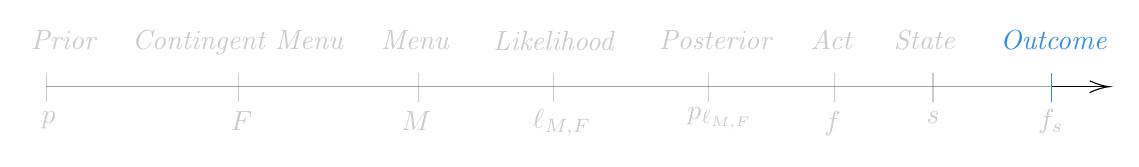
\begin{tikzpicture}[x=0.65pt,y=0.65pt,yscale=-1,xscale=1]
		% Uncomment if required: \path (0,472); % Set diagram left start at 0, and has height of 472

		% Draw the transparent horizontal line (arrow)
		\draw[opacity=0.2] (23,250) -- (614,250);

		% Draw the part of the horizontal arrow to the left of the vertical segment in transparent
		\draw[opacity=0.2] (23,250) -- (582,250);

		% Draw the part of the horizontal arrow to the right of the vertical segment in black
		\draw[black] (582,250) -- (614,250);

		% Draw the black oblique segments at the end of the horizontal arrow (pointing left)
		\draw[black, shift={(614,250)}, rotate=180]
		(10.93,-3.29) .. controls (6.95,-1.4) and (3.31,-0.3) .. (0,0) .. controls (3.31,0.3) and (6.95,1.4) .. (10.93,3.29);

		% Draw the small vertical segments below each word
		\draw[opacity=0.2] (23,242.5) -- (23,258.5);
		\draw[opacity=0.2] (130,242.5) -- (130,258.5);
		\draw[opacity=0.2] (230,242.5) -- (230,258.5);
		\draw[opacity=0.2] (305,242.5) -- (305,258.5);
		\draw[opacity=0.2] (391,242.5) -- (391,258.5);
		\draw[opacity=0.2] (461,242.5) -- (461,258.5);
		\draw[opacity=0.2] (516,242.5) -- (516,258.5);

		% The vertical segment below "Outcome" in blue
		\draw[opacity=1, blue] (582,242.5) -- (582,258.5);

		% Text for symbols (bottom) with reduced opacity
		\draw[opacity=0.2] (124,262.15) node [anchor=north west][inner sep=0.75pt] {\( F \)};
		\draw[opacity=0.2] (219,262.15) node [anchor=north west][inner sep=0.75pt] {\(M\)};
		\draw[opacity=0.2] (378,260.15) node [anchor=north west][inner sep=0.75pt] {\(p_{\ell_{M,F}}\)};
		\draw[opacity=0.2] (511,262.15) node [anchor=north west][inner sep=0.75pt] {\(s\)};
		\draw[opacity=0.2] (573,261.15) node [anchor=north west][inner sep=0.75pt] {\(f_{s}\)};
		\draw[opacity=0.2] (454,262.15) node [anchor=north west][inner sep=0.75pt] {\(f\)};
		\draw[opacity=0.2] (292,261.15) node [anchor=north west][inner sep=0.75pt] {\(\ell_{M,F}\)};
		\draw[opacity=0.2] (19,262.15) node [anchor=north west][inner sep=0.75pt] {\(p\)};

		% Text for labels (top) with reduced opacity
		\draw[opacity=0.2] (69.29,217.5) node [anchor=north west][inner sep=0.75pt] [align=left] {\textit{Contingent Menu}};
		\draw[opacity=0.2] (207.58,217.5) node [anchor=north west][inner sep=0.75pt] [align=left] {\textit{Menu}};
		\draw[opacity=0.2] (362.16,217.5) node [anchor=north west][inner sep=0.75pt] [align=left] {\textit{Posterior}};
		\draw[opacity=0.2] (492.74,217.5) node [anchor=north west][inner sep=0.75pt] [align=left] {\textit{State}};
		\draw[opacity=0.2] (446.45,217.5) node [anchor=north west][inner sep=0.75pt] [align=left] {\textit{Act}};
		\draw[opacity=0.2] (269.87,217.5) node [anchor=north west][inner sep=0.75pt] [align=left] {\textit{Likelihood}};
		\draw[opacity=0.2] (13,217.5) node [anchor=north west][inner sep=0.75pt] [align=left] {\textit{Prior}};

		% The word "Outcome" in blue
		\draw[opacity=1, blue] (552,217.5) node [anchor=north west][inner sep=0.75pt] [align=left] {\textit{Outcome}};
	\end{tikzpicture}

	\vfill

	\begin{columns}
		% Left Column (adjusted width and smaller table font)
		\begin{column}{0.45\textwidth}  % Increased width slightly to 0.45\textwidth
			\begin{center}
				%\scriptsize  % Reduces the font size inside the table
				\begin{table}[H]
					\centering
					\begin{tabular}{c | c}
						\multicolumn{2}{c}{}                        \\
						State  & Menus                              \\
						\hline
						Good   & \multirow{2}{*}{ \( i_{p}, w_p \)} \\
						Normal &                                    \\
						Bad    & \(  i_{q}, w_q \)                  \\
					\end{tabular}
					%\caption{Menus and Contingent Menus.}
					%\label{tab:actions_inv1}
				\end{table}
			\end{center}
		\end{column}

		% Right Column (slightly reduced width)
		\begin{column}{0.55\textwidth}  % Adjusted right column to 0.55\textwidth
			\begin{itemize}
				\item \textcolor{blue}{outcome} set (net financial gains);
			\end{itemize}
		\end{column}
	\end{columns}

\end{frame}

\begin{frame}[noframenumbering]{Model: acts}

	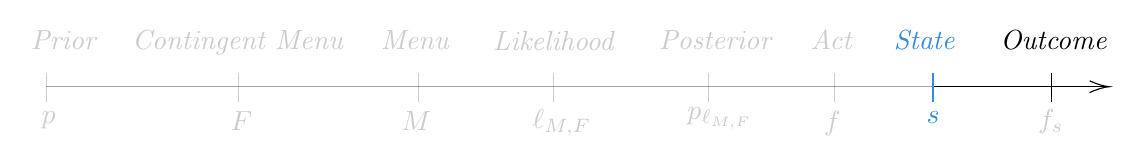
\begin{tikzpicture}[x=0.65pt,y=0.65pt,yscale=-1,xscale=1]
		% Uncomment if required: \path (0,472); % Set diagram left start at 0, and has height of 472

		% Draw the transparent horizontal line (arrow)
		\draw[opacity=0.2] (23,250) -- (614,250);

		% Draw the part of the horizontal arrow to the left of the vertical segment in transparent
		\draw[opacity=0.2] (23,250) -- (582,250);

		% Draw the part of the horizontal arrow to the right of the vertical segment in black
		\draw[black] (516,250) -- (614,250);

		% Draw the black oblique segments at the end of the horizontal arrow (pointing left)
		\draw[black, shift={(614,250)}, rotate=180]
		(10.93,-3.29) .. controls (6.95,-1.4) and (3.31,-0.3) .. (0,0) .. controls (3.31,0.3) and (6.95,1.4) .. (10.93,3.29);

		% Draw the small vertical segments below each word
		\draw[opacity=0.2] (23,242.5) -- (23,258.5);
		\draw[opacity=0.2] (130,242.5) -- (130,258.5);
		\draw[opacity=0.2] (230,242.5) -- (230,258.5);
		\draw[opacity=0.2] (305,242.5) -- (305,258.5);
		\draw[opacity=0.2] (391,242.5) -- (391,258.5);
		\draw[opacity=0.2] (461,242.5) -- (461,258.5);

		% The vertical segment below "Outcome" in black
		\draw[black] (582,242.5) -- (582,258.5);

		% The word "Outcome" in black
		\draw[opacity=1, black] (552,217.5) node [anchor=north west][inner sep=0.75pt] [align=left] {\textit{Outcome}};

		% The vertical segment below "State" in blue
		\draw[opacity=1, blue] (516,242.5) -- (516,258.5);

		% The word "State" in blue
		\draw[opacity=1, blue] (492.74,217.5) node [anchor=north west][inner sep=0.75pt] [align=left] {\textit{State}};

		% The symbol "s" in blue
		\draw[opacity=1, blue] (511,262.15) node [anchor=north west][inner sep=0.75pt] {\(s\)};

		% Text for symbols (bottom) with reduced opacity
		\draw[opacity=0.2] (124,262.15) node [anchor=north west][inner sep=0.75pt] {\( F \)};
		\draw[opacity=0.2] (219,262.15) node [anchor=north west][inner sep=0.75pt] {\(M\)};
		\draw[opacity=0.2] (378,260.15) node [anchor=north west][inner sep=0.75pt] {\(p_{\ell_{M,F}}\)};
		\draw[opacity=0.2] (573,261.15) node [anchor=north west][inner sep=0.75pt] {\(f_{s}\)};
		\draw[opacity=0.2] (454,262.15) node [anchor=north west][inner sep=0.75pt] {\(f\)};
		\draw[opacity=0.2] (292,261.15) node [anchor=north west][inner sep=0.75pt] {\(\ell_{M,F}\)};
		\draw[opacity=0.2] (19,262.15) node [anchor=north west][inner sep=0.75pt] {\(p\)};

		% Text for labels (top) with reduced opacity
		\draw[opacity=0.2] (69.29,217.5) node [anchor=north west][inner sep=0.75pt] [align=left] {\textit{Contingent Menu}};
		\draw[opacity=0.2] (207.58,217.5) node [anchor=north west][inner sep=0.75pt] [align=left] {\textit{Menu}};
		\draw[opacity=0.2] (362.16,217.5) node [anchor=north west][inner sep=0.75pt] [align=left] {\textit{Posterior}};
		\draw[opacity=0.2] (446.45,217.5) node [anchor=north west][inner sep=0.75pt] [align=left] {\textit{Act}};
		\draw[opacity=0.2] (269.87,217.5) node [anchor=north west][inner sep=0.75pt] [align=left] {\textit{Likelihood}};
		\draw[opacity=0.2] (13,217.5) node [anchor=north west][inner sep=0.75pt] [align=left] {\textit{Prior}};
	\end{tikzpicture}


	\vfill

	\begin{columns}
		% Left Column (adjusted width and smaller table font)
		\begin{column}{0.45\textwidth}  % Increased width slightly to 0.45\textwidth
			\begin{center}
				%\scriptsize  % Reduces the font size inside the table
				\begin{table}[H]
					\centering
					\begin{tabular}{c | c}
						\multicolumn{2}{c}{}                                          \\
						State                    & Menu                               \\
						\hline
						\textcolor{blue}{Good}   & \multirow{2}{*}{\( i_{p}, w_p \) } \\
						\textcolor{blue}{Normal} &                                    \\
						\textcolor{blue}{Bad}    & \( i_{q}, w_q \)                   \\
					\end{tabular}
					%\caption{Menus and Contingent Menus.}
					%\label{tab:actions_inv}
				\end{table}
			\end{center}
		\end{column}

		% Right Column (slightly reduced width)
		\begin{column}{0.55\textwidth}  % Adjusted right column to 0.55\textwidth
			\begin{itemize}
				\item outcome set;
				\item \textcolor{blue}{state} set;
			\end{itemize}
		\end{column}
	\end{columns}

\end{frame}

\begin{frame}[noframenumbering]{Model: acts}

	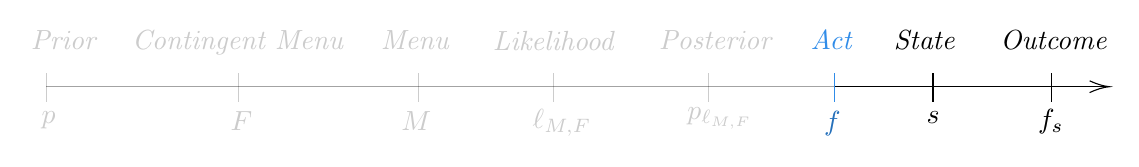
\begin{tikzpicture}[x=0.65pt,y=0.65pt,yscale=-1,xscale=1]
		% Uncomment if required: \path (0,472); % Set diagram left start at 0, and has height of 472

		% Draw the transparent horizontal line (arrow)
		\draw[opacity=0.2] (23,250) -- (614,250);

		% Draw the part of the horizontal arrow to the left of the vertical segment in transparent
		\draw[opacity=0.2] (23,250) -- (582,250);

		% Draw the part of the horizontal arrow to the right of the vertical segment in black
		\draw[black] (461,250) -- (614,250);

		% Draw the black oblique segments at the end of the horizontal arrow (pointing left)
		\draw[black, shift={(614,250)}, rotate=180]
		(10.93,-3.29) .. controls (6.95,-1.4) and (3.31,-0.3) .. (0,0) .. controls (3.31,0.3) and (6.95,1.4) .. (10.93,3.29);

		% Draw the small vertical segments below each word
		\draw[opacity=0.2] (23,242.5) -- (23,258.5);
		\draw[opacity=0.2] (130,242.5) -- (130,258.5);
		\draw[opacity=0.2] (230,242.5) -- (230,258.5);
		\draw[opacity=0.2] (305,242.5) -- (305,258.5);
		\draw[opacity=0.2] (391,242.5) -- (391,258.5);

		% The vertical segment below "Outcome, State" in black
		\draw[black] (582,242.5) -- (582,258.5);
		\draw[black] (516,242.5) -- (516,258.5);

		% The word "Outcome, State" in black
		\draw[opacity=1, black] (552,217.5) node [anchor=north west][inner sep=0.75pt] [align=left] {\textit{Outcome}};
		\draw[opacity=1, black] (492.74,217.5) node [anchor=north west][inner sep=0.75pt] [align=left] {\textit{State}};

		% The vertical segment below "Act" in blue
		\draw[opacity=1, blue] (461,242.5) -- (461,258.5);

		% The word "Act" in blue
		\draw[opacity=1, blue] (446.45,217.5) node [anchor=north west][inner sep=0.75pt] [align=left] {\textit{Act}};

		% The symbol "s, f_s" in black
		\draw[opacity=1, black] (511,262.15) node [anchor=north west][inner sep=0.75pt] {\(s\)};
		\draw[opacity=1, black] (573,261.15) node [anchor=north west][inner sep=0.75pt] {\(f_{s}\)};

		% The symbol "f" in blue
		\draw[opacity=1, blue] (454,262.15) node [anchor=north west][inner sep=0.75pt] {\(f\)};

		% Text for symbols (bottom) with reduced opacity
		\draw[opacity=0.2] (124,262.15) node [anchor=north west][inner sep=0.75pt] {\( F \)};
		\draw[opacity=0.2] (219,262.15) node [anchor=north west][inner sep=0.75pt] {\(M\)};
		\draw[opacity=0.2] (378,260.15) node [anchor=north west][inner sep=0.75pt] {\(p_{\ell_{M,F}}\)};
		\draw[opacity=0.2] (573,261.15) node [anchor=north west][inner sep=0.75pt] {\(f_{s}\)};
		\draw[opacity=0.2] (454,262.15) node [anchor=north west][inner sep=0.75pt] {\(f\)};
		\draw[opacity=0.2] (292,261.15) node [anchor=north west][inner sep=0.75pt] {\(\ell_{M,F}\)};
		\draw[opacity=0.2] (19,262.15) node [anchor=north west][inner sep=0.75pt] {\(p\)};

		% Text for labels (top) with reduced opacity
		\draw[opacity=0.2] (69.29,217.5) node [anchor=north west][inner sep=0.75pt] [align=left] {\textit{Contingent Menu}};
		\draw[opacity=0.2] (207.58,217.5) node [anchor=north west][inner sep=0.75pt] [align=left] {\textit{Menu}};
		\draw[opacity=0.2] (362.16,217.5) node [anchor=north west][inner sep=0.75pt] [align=left] {\textit{Posterior}};
		\draw[opacity=0.2] (269.87,217.5) node [anchor=north west][inner sep=0.75pt] [align=left] {\textit{Likelihood}};
		\draw[opacity=0.2] (13,217.5) node [anchor=north west][inner sep=0.75pt] [align=left] {\textit{Prior}};
	\end{tikzpicture}

	\vfill

	\begin{columns}
		% Left Column (adjusted width and smaller table font)
		\begin{column}{0.45\textwidth}  % Increased width slightly to 0.45\textwidth
			\begin{center}
				%\scriptsize  % Reduces the font size inside the table
				\begin{table}[H]
					\centering
					\begin{tabular}{c | c}
						\multicolumn{2}{c}{}                                       \\
						State  & Menu                                              \\
						\hline
						Good   & \multirow{2}{*}{\( \textcolor{blue}{i_p}, w_p \)} \\
						Normal &                                                   \\
						Bad    & \(i_q , w_q \)                                    \\
					\end{tabular}

					%\caption{Menus and Contingent Menus.}
					%\label{tab:actions_inv3}
				\end{table}
			\end{center}
		\end{column}

		% Right Column (slightly reduced width)
		\begin{column}{0.55\textwidth}  % Adjusted right column to 0.55\textwidth
			\begin{itemize}
				\item outcome set;
				\item state set ;
				\item \textcolor{blue}{acts} \( f : \: States \: \rightarrow \: Outcomes \);
			\end{itemize}
		\end{column}
	\end{columns}

\end{frame}

\begin{frame}{Model: menus and contingent menus}

	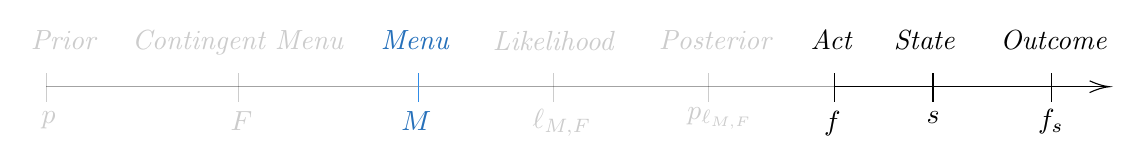
\begin{tikzpicture}[x=0.65pt,y=0.65pt,yscale=-1,xscale=1]
		% Uncomment if required: \path (0,472); % Set diagram left start at 0, and has height of 472

		% Draw the transparent horizontal line (arrow)
		\draw[opacity=0.2] (23,250) -- (614,250);

		% Draw the part of the horizontal arrow to the left of the vertical segment in transparent
		\draw[opacity=0.2] (23,250) -- (582,250);

		% Draw the part of the horizontal arrow to the right of the vertical segment in black
		\draw[black] (461,250) -- (614,250);

		% Draw the black oblique segments at the end of the horizontal arrow (pointing left)
		\draw[black, shift={(614,250)}, rotate=180]
		(10.93,-3.29) .. controls (6.95,-1.4) and (3.31,-0.3) .. (0,0) .. controls (3.31,0.3) and (6.95,1.4) .. (10.93,3.29);

		% Draw the small vertical segments below each word
		\draw[opacity=0.2] (23,242.5) -- (23,258.5);
		\draw[opacity=0.2] (130,242.5) -- (130,258.5);
		\draw[opacity=0.2] (230,242.5) -- (230,258.5);
		\draw[opacity=0.2] (305,242.5) -- (305,258.5);
		\draw[opacity=0.2] (391,242.5) -- (391,258.5);

		% The vertical segment below "Outcome, State, Act" in black
		\draw[black] (582,242.5) -- (582,258.5);
		\draw[black] (516,242.5) -- (516,258.5);
		\draw[black] (461,242.5) -- (461,258.5);

		% The word "Outcome, State, Act" in black
		\draw[opacity=1, black] (552,217.5) node [anchor=north west][inner sep=0.75pt] [align=left] {\textit{Outcome}};
		\draw[opacity=1, black] (492.74,217.5) node [anchor=north west][inner sep=0.75pt] [align=left] {\textit{State}};
		\draw[opacity=1, black] (446.45,217.5) node [anchor=north west][inner sep=0.75pt] [align=left] {\textit{Act}};

		% The vertical segment below "Menu" in blue
		\draw[opacity=1, blue] (230,242.5) -- (230,258.5);

		% The word "Menu" in blue
		\draw[opacity=1, blue] (207.58,217.5) node [anchor=north west][inner sep=0.75pt] [align=left] {\textit{Menu}};

		% The symbol "s, f_s, f" in black
		\draw[opacity=1, black] (511,262.15) node [anchor=north west][inner sep=0.75pt] {\(s\)};
		\draw[opacity=1, black] (573,261.15) node [anchor=north west][inner sep=0.75pt] {\(f_{s}\)};
		\draw[opacity=1, black] (454,262.15) node [anchor=north west][inner sep=0.75pt] {\(f\)};

		% The symbol "M" in blue
		\draw[opacity=1, blue] (219,262.15) node [anchor=north west][inner sep=0.75pt] {\(M\)};

		% Text for symbols (bottom) with reduced opacity
		\draw[opacity=0.2] (124,262.15) node [anchor=north west][inner sep=0.75pt] {\( F \)};
		\draw[opacity=0.2] (219,262.15) node [anchor=north west][inner sep=0.75pt] {\(M\)};
		\draw[opacity=0.2] (378,260.15) node [anchor=north west][inner sep=0.75pt] {\(p_{\ell_{M,F}}\)};
		\draw[opacity=0.2] (573,261.15) node [anchor=north west][inner sep=0.75pt] {\(f_{s}\)};
		\draw[opacity=0.2] (454,262.15) node [anchor=north west][inner sep=0.75pt] {\(f\)};
		\draw[opacity=0.2] (292,261.15) node [anchor=north west][inner sep=0.75pt] {\(\ell_{M,F}\)};
		\draw[opacity=0.2] (19,262.15) node [anchor=north west][inner sep=0.75pt] {\(p\)};

		% Text for labels (top) with reduced opacity
		\draw[opacity=0.2] (69.29,217.5) node [anchor=north west][inner sep=0.75pt] [align=left] {\textit{Contingent Menu}};
		\draw[opacity=0.2] (207.58,217.5) node [anchor=north west][inner sep=0.75pt] [align=left] {\textit{Menu}};
		\draw[opacity=0.2] (362.16,217.5) node [anchor=north west][inner sep=0.75pt] [align=left] {\textit{Posterior}};
		\draw[opacity=0.2] (269.87,217.5) node [anchor=north west][inner sep=0.75pt] [align=left] {\textit{Likelihood}};
		\draw[opacity=0.2] (13,217.5) node [anchor=north west][inner sep=0.75pt] [align=left] {\textit{Prior}};
	\end{tikzpicture}

	\vfill

	\begin{columns}
		% Left Column (adjusted width and smaller table font)
		\begin{column}{0.45\textwidth}  % Increased width slightly to 0.45\textwidth
			\begin{center}
				%\scriptsize  % Reduces the font size inside the table
				\begin{table}[H]
					\centering
					\begin{tabular}{c | c}
						\multicolumn{2}{c}{}                                       \\
						State  & Menu                                              \\
						\hline
						Good   & \multirow{2}{*}{\textcolor{blue}{\( i_p, w_p \)}} \\
						Normal &                                                   \\
						Bad    & \( i_q, w_q \)                                    \\
					\end{tabular}
					%\caption{Menus and Contingent Menus.}
					%\label{tab:menus2}
				\end{table}
			\end{center}
		\end{column}

		% Right Column (slightly reduced width)
		\begin{column}{0.55\textwidth}  % Adjusted right column to 0.55\textwidth
			\begin{itemize}
				\item outcome set;
				\item state set;
				\item acts \( f : \: States \: \rightarrow \: Outcomes \);
				\item a set of acts is a \textcolor{blue}{menu} \( M \);
			\end{itemize}
		\end{column}
	\end{columns}

\end{frame}

\begin{frame}[noframenumbering]{Model: menus and contingent menus}

	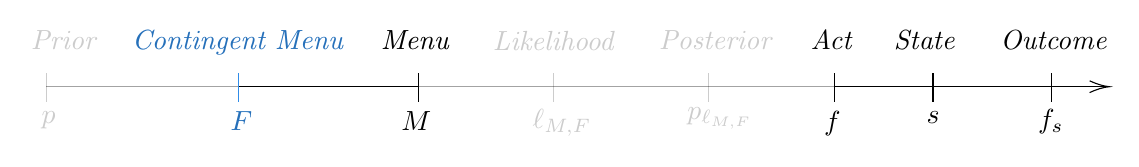
\begin{tikzpicture}[x=0.65pt,y=0.65pt,yscale=-1,xscale=1]
		% Uncomment if required: \path (0,472); % Set diagram left start at 0, and has height of 472

		% Draw the transparent horizontal line (arrow)
		\draw[opacity=0.2] (23,250) -- (614,250);

		% Draw the part of the horizontal arrow to the left of the vertical segment in transparent
		\draw[opacity=0.2] (23,250) -- (582,250);

		% Draw the part of the horizontal arrow to the right of the vertical segment in black
		\draw[black] (130,250) -- (230,250);
		\draw[black] (461,250) -- (614,250);

		% Draw the black oblique segments at the end of the horizontal arrow (pointing left)
		\draw[black, shift={(614,250)}, rotate=180]
		(10.93,-3.29) .. controls (6.95,-1.4) and (3.31,-0.3) .. (0,0) .. controls (3.31,0.3) and (6.95,1.4) .. (10.93,3.29);

		% Draw the small vertical segments below each word
		\draw[opacity=0.2] (23,242.5) -- (23,258.5);
		\draw[opacity=0.2] (130,242.5) -- (130,258.5);
		\draw[opacity=0.2] (230,242.5) -- (230,258.5);
		\draw[opacity=0.2] (305,242.5) -- (305,258.5);
		\draw[opacity=0.2] (391,242.5) -- (391,258.5);

		% The vertical segment below "Outcome, State, Act, Menu" in black
		\draw[black] (582,242.5) -- (582,258.5);
		\draw[black] (516,242.5) -- (516,258.5);
		\draw[black] (461,242.5) -- (461,258.5);
		\draw[black] (230,242.5) -- (230,258.5);

		% The word "Outcome, State, Act, Menu" in black
		\draw[opacity=1, black] (552,217.5) node [anchor=north west][inner sep=0.75pt] [align=left] {\textit{Outcome}};
		\draw[opacity=1, black] (492.74,217.5) node [anchor=north west][inner sep=0.75pt] [align=left] {\textit{State}};
		\draw[opacity=1, black] (446.45,217.5) node [anchor=north west][inner sep=0.75pt] [align=left] {\textit{Act}};
		\draw[opacity=1, black] (207.58,217.5) node [anchor=north west][inner sep=0.75pt] [align=left] {\textit{Menu}};

		% The vertical segment below "Contingent Menu" in blue
		\draw[opacity=1, blue] (130,242.5) -- (130,258.5);

		% The word "Contingent Menu" in blue
		\draw[opacity=1, blue] (69.29,217.5) node [anchor=north west][inner sep=0.75pt] [align=left] {\textit{Contingent Menu}};

		% The symbol "s, f_s, f, M" in black
		\draw[opacity=1, black] (511,262.15) node [anchor=north west][inner sep=0.75pt] {\(s\)};
		\draw[opacity=1, black] (573,261.15) node [anchor=north west][inner sep=0.75pt] {\(f_{s}\)};
		\draw[opacity=1, black] (454,262.15) node [anchor=north west][inner sep=0.75pt] {\(f\)};
		\draw[opacity=1, black] (219,262.15) node [anchor=north west][inner sep=0.75pt] {\(M\)};

		% The symbol "F" in blue
		\draw[opacity=1, blue] (124,262.15) node [anchor=north west][inner sep=0.75pt] {\( F \)};

		% Text for symbols (bottom) with reduced opacity
		\draw[opacity=0.2] (124,262.15) node [anchor=north west][inner sep=0.75pt] {\( F \)};
		\draw[opacity=0.2] (378,260.15) node [anchor=north west][inner sep=0.75pt] {\(p_{\ell_{M,F}}\)};
		\draw[opacity=0.2] (292,261.15) node [anchor=north west][inner sep=0.75pt] {\(\ell_{M,F}\)};
		\draw[opacity=0.2] (19,262.15) node [anchor=north west][inner sep=0.75pt] {\(p\)};

		% Text for labels (top) with reduced opacity
		\draw[opacity=0.2] (69.29,217.5) node [anchor=north west][inner sep=0.75pt] [align=left] {\textit{Contingent Menu}};
		\draw[opacity=0.2] (207.58,217.5) node [anchor=north west][inner sep=0.75pt] [align=left] {\textit{Menu}};
		\draw[opacity=0.2] (362.16,217.5) node [anchor=north west][inner sep=0.75pt] [align=left] {\textit{Posterior}};
		\draw[opacity=0.2] (269.87,217.5) node [anchor=north west][inner sep=0.75pt] [align=left] {\textit{Likelihood}};
		\draw[opacity=0.2] (13,217.5) node [anchor=north west][inner sep=0.75pt] [align=left] {\textit{Prior}};
	\end{tikzpicture}

	\vfill

	\begin{columns}
		% Left Column (adjusted width and smaller table font)
		\begin{column}{0.45\textwidth}  % Increased width slightly to 0.45\textwidth
			\begin{center}
				%\scriptsize  % Reduces the font size inside the table

				\begin{table}[H]
					\centering
					\begin{tabular}{c | c}
						\multicolumn{2}{c}{}                                                         \\
						\textcolor{blue}{State}  & \textcolor{blue}{Menu}                            \\
						\hline
						\textcolor{blue}{Good}   & \textcolor{blue}{\multirow{2}{*}{\( i_p, w_p \)}} \\
						\textcolor{blue}{Normal} & \textcolor{blue}{}                                \\
						\textcolor{blue}{Bad}    & \textcolor{blue}{\( i_q, w_q \)}                  \\
					\end{tabular}
					%\caption{Menus and Contingent Menus.}
					%\label{tab:menus3}
				\end{table}
			\end{center}
		\end{column}

		% Right Column (slightly reduced width)
		\begin{column}{0.55\textwidth}  % Adjusted right column to 0.55\textwidth
			\begin{itemize}
				\item outcome set;
				\item state set;
				\item acts \( f : \: States \: \rightarrow \: Outcomes \);
				\item a set of acts is a menu \( M \);
				\item a \textcolor{blue}{contingent menu} is \(F: States \: \rightarrow \: Menus \).
			\end{itemize}
		\end{column}
	\end{columns}

\end{frame}

\begin{frame}{Information}

	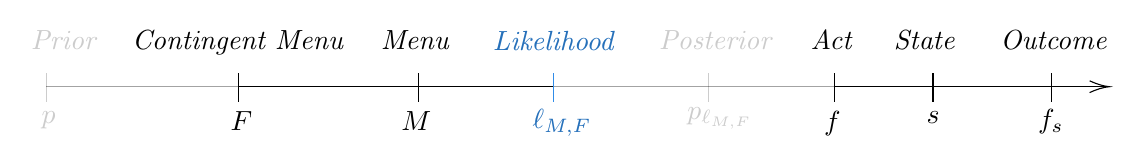
\begin{tikzpicture}[x=0.65pt,y=0.65pt,yscale=-1,xscale=1]
		% Uncomment if required: \path (0,472); % Set diagram left start at 0, and has height of 472

		% Draw the transparent horizontal line (arrow)
		\draw[opacity=0.2] (23,250) -- (614,250);

		% Draw the part of the horizontal arrow to the left of the vertical segment in transparent
		\draw[opacity=0.2] (23,250) -- (582,250);

		% Draw the part of the horizontal arrow to the right of the vertical segment in black
		\draw[black] (130,250) -- (305,250);
		\draw[black] (461,250) -- (614,250);

		% Draw the black oblique segments at the end of the horizontal arrow (pointing left)
		\draw[black, shift={(614,250)}, rotate=180]
		(10.93,-3.29) .. controls (6.95,-1.4) and (3.31,-0.3) .. (0,0) .. controls (3.31,0.3) and (6.95,1.4) .. (10.93,3.29);

		% Draw the small vertical segments below each word
		\draw[opacity=0.2] (23,242.5) -- (23,258.5);
		\draw[opacity=0.2] (130,242.5) -- (130,258.5);
		\draw[opacity=0.2] (230,242.5) -- (230,258.5);
		\draw[opacity=0.2] (305,242.5) -- (305,258.5);
		\draw[opacity=0.2] (391,242.5) -- (391,258.5);

		% The vertical segment below "Outcome, State, Act, Menu, Contingent Menu" in black
		\draw[black] (582,242.5) -- (582,258.5);
		\draw[black] (516,242.5) -- (516,258.5);
		\draw[black] (461,242.5) -- (461,258.5);
		\draw[black] (230,242.5) -- (230,258.5);
		\draw[black] (130,242.5) -- (130,258.5);

		% The word "Outcome, State, Act, Menu, Contingent Menu" in black
		\draw[opacity=1, black] (552,217.5) node [anchor=north west][inner sep=0.75pt] [align=left] {\textit{Outcome}};
		\draw[opacity=1, black] (492.74,217.5) node [anchor=north west][inner sep=0.75pt] [align=left] {\textit{State}};
		\draw[opacity=1, black] (446.45,217.5) node [anchor=north west][inner sep=0.75pt] [align=left] {\textit{Act}};
		\draw[opacity=1, black] (207.58,217.5) node [anchor=north west][inner sep=0.75pt] [align=left] {\textit{Menu}};
		\draw[opacity=1, black] (69.29,217.5) node [anchor=north west][inner sep=0.75pt] [align=left] {\textit{Contingent Menu}};

		% The vertical segment below "Likelihood" in blue
		\draw[opacity=1, blue] (305,242.5) -- (305,258.5);

		% The word "Likelihood" in blue
		\draw[opacity=1, blue] (269.87,217.5) node [anchor=north west][inner sep=0.75pt] [align=left] {\textit{Likelihood}};

		% The symbol "s, f_s, f, M, F" in black
		\draw[opacity=1, black] (511,262.15) node [anchor=north west][inner sep=0.75pt] {\(s\)};
		\draw[opacity=1, black] (573,261.15) node [anchor=north west][inner sep=0.75pt] {\(f_{s}\)};
		\draw[opacity=1, black] (454,262.15) node [anchor=north west][inner sep=0.75pt] {\(f\)};
		\draw[opacity=1, black] (219,262.15) node [anchor=north west][inner sep=0.75pt] {\(M\)};
		\draw[opacity=1, black] (124,262.15) node [anchor=north west][inner sep=0.75pt] {\( F \)};

		% The symbol "\ell_m,f" in blue
		\draw[opacity=1, blue] (292,261.15) node [anchor=north west][inner sep=0.75pt] {\(\ell_{M,F}\)};

		% Text for symbols (bottom) with reduced opacity
		\draw[opacity=0.2] (378,260.15) node [anchor=north west][inner sep=0.75pt] {\(p_{\ell_{M,F}}\)};
		\draw[opacity=0.2] (292,261.15) node [anchor=north west][inner sep=0.75pt] {\(\ell_{M,F}\)};
		\draw[opacity=0.2] (19,262.15) node [anchor=north west][inner sep=0.75pt] {\(p\)};

		% Text for labels (top) with reduced opacity
		\draw[opacity=0.2] (362.16,217.5) node [anchor=north west][inner sep=0.75pt] [align=left] {\textit{Posterior}};
		\draw[opacity=0.2] (269.87,217.5) node [anchor=north west][inner sep=0.75pt] [align=left] {\textit{Likelihood}};
		\draw[opacity=0.2] (13,217.5) node [anchor=north west][inner sep=0.75pt] [align=left] {\textit{Prior}};
	\end{tikzpicture}

	\vfill

	\begin{columns}
		% Left Column (adjusted width)
		\begin{column}{0.35\textwidth} % Reduced width to make room for the right column
			\begin{center}
				\begin{table}
					\centering
					\begin{tabular}{c | c}
						\multicolumn{2}{c}{}                                                                \\
						State  & Menu                                                                       \\
						\hline
						Good   & \multirow{2}{*}{\( \textcolor{blue}{1} \cdot \left\{ i_p, w_p \right\} \)} \\
						Normal &                                                                            \\
						Bad    & \( \textcolor{blue}{1} \cdot \left\{ i_q, w_q \right\}\)                   \\
					\end{tabular}
					%\caption{Information.}
					%\label{tab:info2}
				\end{table}
			\end{center}
		\end{column}

		% Right Column (adjusted width to take up more space)
		\begin{column}{0.65\textwidth} % Increased width to make room for the content
			\begin{itemize}
				\item a contingent menu is \(F: States \: \rightarrow \: Menus \);
				\item probability menu \( M \) realises in state \( s \) is \( \textcolor{blue}{F_s \left( M \right)} \); \pause
			\end{itemize}
		\end{column}
	\end{columns}

	\vspace{0.6cm}

	The likelihood of state \(s\) after realisation of menu \(M\) from the contingent menu \(F\) is

	\vfill

	\[ \ell_{M, F} \left( Good \right) = \frac{1}{1+1} = \frac{1}{2} .
	\]

\end{frame}

\begin{frame}[noframenumbering]{Information}

	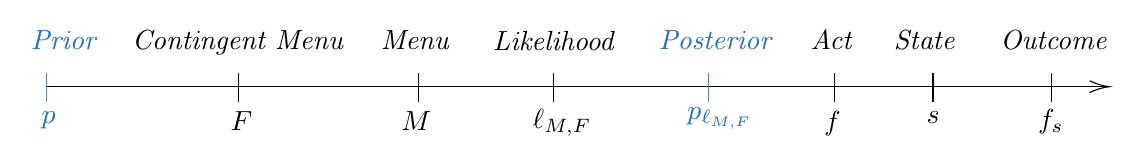
\begin{tikzpicture}[x=0.65pt,y=0.65pt,yscale=-1,xscale=1]
		% Uncomment if required: \path (0,472); % Set diagram left start at 0, and has height of 472

		% Draw the transparent horizontal line (arrow)
		\draw[opacity=0.2] (23,250) -- (614,250);

		% Draw the part of the horizontal arrow to the left of the vertical segment in transparent
		\draw[opacity=0.2] (23,250) -- (582,250);

		% Draw the part of the horizontal arrow to the right of the vertical segment in black
		\draw[black] (23,250) -- (461,250);
		\draw[black] (461,250) -- (614,250);

		% Draw the black oblique segments at the end of the horizontal arrow (pointing left)
		\draw[black, shift={(614,250)}, rotate=180]
		(10.93,-3.29) .. controls (6.95,-1.4) and (3.31,-0.3) .. (0,0) .. controls (3.31,0.3) and (6.95,1.4) .. (10.93,3.29);

		% Draw the small vertical segments below each word
		\draw[opacity=0.2] (23,242.5) -- (23,258.5);
		\draw[opacity=0.2] (130,242.5) -- (130,258.5);
		\draw[opacity=0.2] (230,242.5) -- (230,258.5);
		\draw[opacity=0.2] (305,242.5) -- (305,258.5);
		\draw[opacity=0.2] (391,242.5) -- (391,258.5);

		% The vertical segment below "Outcome, State, Act, Menu, Contingent Menu, Likelihood" in black
		\draw[black] (582,242.5) -- (582,258.5);
		\draw[black] (516,242.5) -- (516,258.5);
		\draw[black] (461,242.5) -- (461,258.5);
		\draw[black] (230,242.5) -- (230,258.5);
		\draw[black] (130,242.5) -- (130,258.5);
		\draw[black] (305,242.5) -- (305,258.5);

		% The word "Outcome, State, Act, Menu, Contingent Menu, Likelihood" in black
		\draw[opacity=1, black] (552,217.5) node [anchor=north west][inner sep=0.75pt] [align=left] {\textit{Outcome}};
		\draw[opacity=1, black] (492.74,217.5) node [anchor=north west][inner sep=0.75pt] [align=left] {\textit{State}};
		\draw[opacity=1, black] (446.45,217.5) node [anchor=north west][inner sep=0.75pt] [align=left] {\textit{Act}};
		\draw[opacity=1, black] (207.58,217.5) node [anchor=north west][inner sep=0.75pt] [align=left] {\textit{Menu}};
		\draw[opacity=1, black] (69.29,217.5) node [anchor=north west][inner sep=0.75pt] [align=left] {\textit{Contingent Menu}};
		\draw[opacity=1, black] (269.87,217.5) node [anchor=north west][inner sep=0.75pt] [align=left] {\textit{Likelihood}};

		% The vertical segment below "Prior, Posterior" in blue
		\draw[opacity=1, blue] (23,242.5) -- (23,258.5);
		\draw[opacity=1, blue] (391,242.5) -- (391,258.5);

		% The word "Prior, Posterior" in blue
		\draw[opacity=1, blue] (362.16,217.5) node [anchor=north west][inner sep=0.75pt] [align=left] {\textit{Posterior}};
		\draw[opacity=1, blue] (13,217.5) node [anchor=north west][inner sep=0.75pt] [align=left] {\textit{Prior}};

		% The symbol "s, f_s, f, M, F, \ell_m,f" in black
		\draw[opacity=1, black] (511,262.15) node [anchor=north west][inner sep=0.75pt] {\(s\)};
		\draw[opacity=1, black] (573,261.15) node [anchor=north west][inner sep=0.75pt] {\(f_{s}\)};
		\draw[opacity=1, black] (454,262.15) node [anchor=north west][inner sep=0.75pt] {\(f\)};
		\draw[opacity=1, black] (219,262.15) node [anchor=north west][inner sep=0.75pt] {\(M\)};
		\draw[opacity=1, black] (124,262.15) node [anchor=north west][inner sep=0.75pt] {\( F \)};
		\draw[opacity=1, black] (292,261.15) node [anchor=north west][inner sep=0.75pt] {\(\ell_{M,F}\)};

		% The symbol "p, p_\ell" in blue
		\draw[opacity=1, blue] (378,260.15) node [anchor=north west][inner sep=0.75pt] {\(p_{\ell_{M,F}}\)};
		\draw[opacity=1, blue] (19,262.15) node [anchor=north west][inner sep=0.75pt] {\(p\)};

		% Text for symbols (bottom) with reduced opacity
		\draw[opacity=0.2] (378,260.15) node [anchor=north west][inner sep=0.75pt] {\(p_{\ell_{M,F}}\)};
		\draw[opacity=0.2] (19,262.15) node [anchor=north west][inner sep=0.75pt] {\(p\)};

		% Text for labels (top) with reduced opacity
		\draw[opacity=0.2] (362.16,217.5) node [anchor=north west][inner sep=0.75pt] [align=left] {\textit{Posterior}};
		\draw[opacity=0.2] (13,217.5) node [anchor=north west][inner sep=0.75pt] [align=left] {\textit{Prior}};
	\end{tikzpicture}

	\vfill

	\begin{columns}
		% Left Column (adjusted width)
		\begin{column}{0.35\textwidth} % Reduced width to make room for the right column
			\begin{center}
				\begin{table}
					\centering
					\begin{tabular}{c | c}
						\multicolumn{2}{c}{}                                                                \\
						State  & Menu                                                                       \\
						\hline
						Good   & \multirow{2}{*}{\( \textcolor{blue}{1} \cdot \left\{ i_p, w_p \right\} \)} \\
						Normal &                                                                            \\
						Bad    & \(\textcolor{blue}{1} \cdot \left\{ i_q, w_q \right\} \)                   \\
					\end{tabular}
					%\caption{Information.}
					%\label{tab:info1}
				\end{table}
			\end{center}
		\end{column}

		% Right Column (adjusted width to take up more space)
		\begin{column}{0.65\textwidth} % Increased width to make room for the content
			\begin{itemize}
				\item a contingent menu is \(F: States \: \rightarrow \: Menus \);
				\item probability menu \( M \) realises in state \( s \) is \( F_s \left( M \right) \);
				\item prior \( \textcolor{blue}{p} \) and likelihood \( \ell_{M,F} \) induce posterior \( \textcolor{blue}{p_{\ell_{M,F}}} \).
			\end{itemize}
		\end{column}
	\end{columns}

	\vspace{0.6cm}

	The likelihood of state \(s\) after realisation of menu \(M\) from the contingent menu \(F\) is

	\vfill

	\[ \ell_{M, F} \left( Good \right) = \frac{1}{1+1} = \frac{1}{2} \hspace{2cm} \ell_{M, F} \left( s \right) = \frac{F_{s} \left( M \right)}{ \sum_{s^{\prime} \in S} F_{s^{\prime}} \left( M \right)} .
	\]

\end{frame}

\begin{frame}{Utility over acts}


	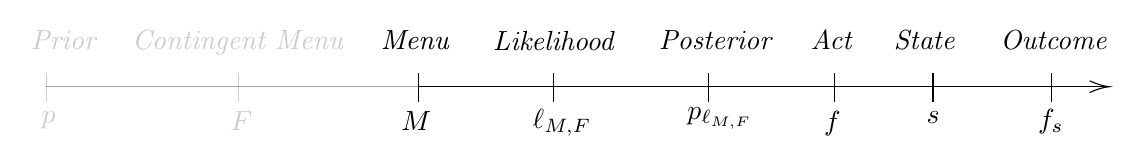
\begin{tikzpicture}[x=0.65pt,y=0.65pt,yscale=-1,xscale=1]
		% Uncomment if required: \path (0,472); % Set diagram left start at 0, and has height of 472

		% Draw the transparent horizontal line (arrow)
		\draw[opacity=0.2] (23,250) -- (614,250);

		% Draw the part of the horizontal arrow to the left of the vertical segment in transparent
		\draw[opacity=0.2] (23,250) -- (582,250);

		% Draw the part of the horizontal arrow to the right of the vertical segment in black
		\draw[black] (230,250) -- (614,250);

		% Draw the black oblique segments at the end of the horizontal arrow (pointing left)
		\draw[black, shift={(614,250)}, rotate=180]
		(10.93,-3.29) .. controls (6.95,-1.4) and (3.31,-0.3) .. (0,0) .. controls (3.31,0.3) and (6.95,1.4) .. (10.93,3.29);

		% Draw the small vertical segments below each word
		\draw[opacity=0.2] (23,242.5) -- (23,258.5);
		\draw[opacity=0.2] (130,242.5) -- (130,258.5);
		\draw[opacity=0.2] (230,242.5) -- (230,258.5);
		\draw[black] (305,242.5) -- (305,258.5);
		\draw[black] (391,242.5) -- (391,258.5);

		% The vertical segment below "Outcome, State, Act" in black
		\draw[black] (582,242.5) -- (582,258.5);
		\draw[black] (516,242.5) -- (516,258.5);
		\draw[black] (461,242.5) -- (461,258.5);

		% The word "Outcome, State, Act" in black
		\draw[opacity=1, black] (552,217.5) node [anchor=north west][inner sep=0.75pt] [align=left] {\textit{Outcome}};
		\draw[opacity=1, black] (492.74,217.5) node [anchor=north west][inner sep=0.75pt] [align=left] {\textit{State}};
		\draw[opacity=1, black] (446.45,217.5) node [anchor=north west][inner sep=0.75pt] [align=left] {\textit{Act}};

		% The vertical segment below "Menu" in blue
		\draw[opacity=1, black] (230,242.5) -- (230,258.5);

		% The word "Menu" in blue
		\draw[opacity=1, black] (207.58,217.5) node [anchor=north west][inner sep=0.75pt] [align=left] {\textit{Menu}};

		% The symbol "s, f_s, f" in black
		\draw[opacity=1, black] (511,262.15) node [anchor=north west][inner sep=0.75pt] {\(s\)};
		\draw[opacity=1, black] (573,261.15) node [anchor=north west][inner sep=0.75pt] {\(f_{s}\)};
		\draw[opacity=1, black] (454,262.15) node [anchor=north west][inner sep=0.75pt] {\(f\)};

		% The symbol "M" in blue
		\draw[opacity=1, black] (219,262.15) node [anchor=north west][inner sep=0.75pt] {\(M\)};

		% Text for symbols (bottom) with reduced opacity
		\draw[opacity=0.2] (124,262.15) node [anchor=north west][inner sep=0.75pt] {\( F \)};
		\draw[opacity=0.2] (219,262.15) node [anchor=north west][inner sep=0.75pt] {\(M\)};
		\draw[opacity=1, black] (378,260.15) node [anchor=north west][inner sep=0.75pt] {\(p_{\ell_{M,F}}\)};
		\draw[opacity=0.2] (573,261.15) node [anchor=north west][inner sep=0.75pt] {\(f_{s}\)};
		\draw[opacity=0.2] (454,262.15) node [anchor=north west][inner sep=0.75pt] {\(f\)};
		\draw[opacity=1, black] (292,261.15) node [anchor=north west][inner sep=0.75pt] {\(\ell_{M,F}\)};
		\draw[opacity=0.2] (19,262.15) node [anchor=north west][inner sep=0.75pt] {\(p\)};

		% Text for labels (top) with reduced opacity
		\draw[opacity=0.2] (69.29,217.5) node [anchor=north west][inner sep=0.75pt] [align=left] {\textit{Contingent Menu}};
		\draw[opacity=0.2] (207.58,217.5) node [anchor=north west][inner sep=0.75pt] [align=left] {\textit{Menu}};
		\draw[opacity=1, black] (362.16,217.5) node [anchor=north west][inner sep=0.75pt] [align=left] {\textit{Posterior}};
		\draw[opacity=1, black] (269.87,217.5) node [anchor=north west][inner sep=0.75pt] [align=left] {\textit{Likelihood}};
		\draw[opacity=0.2] (13,217.5) node [anchor=north west][inner sep=0.75pt] [align=left] {\textit{Prior}};
	\end{tikzpicture}

	\vspace{0.2cm}

	\begin{center}  % Center the columns in the overall slide
		\begin{columns}
			% Left Column (adjusted width and smaller table font)
			\begin{column}{0.5\textwidth}
				Expected utility of act \( f \) at likelihood \( \ell_{M, F} \)
				\vfill
				\[
					\sum_{s} p_{\ell_{M, F}} \left( s \right) u \left( f_{s} ; \ell_{M, F} \right) .
				\]
				\pause
			\end{column}

			% Right Column (slightly reduced width)
			\begin{column}{0.5\textwidth}
				Under distorted likelihood \( \textcolor{blue}{\ell^{*}_{M,F}} \)
				\vfill
				\[
					\sum_{s} p_{\textcolor{blue}{\ell^{*}_{M, F}}} \left( s \right) u \left( f_{s} ; \textcolor{blue}{\ell^{*}_{M, F}} \right).
				\]
				\pause
			\end{column}
		\end{columns}
	\end{center}

	\vfill

	The main theorem identifies conditions under which the individual solves

	\vfill

	\[
		\max _{f \in M} \left[ \underbrace{\sum_{s} p_{\ell_{M, F}}(s) u \left( f_{s}; \ell_{M, F} \right)}_{\text{\textit{EU}}} +
			\alpha_{\ell_{M, F}} \underbrace{\sum_{s} p_{\textcolor{blue}{\ell^{*}_{M, F}}} \left( s \right) u \left( f_{s} ; \textcolor{blue}{\ell^{*}_{M, F}} \right)}_{\text{\textit{distorted EU}}} \right] .
	\]

\end{frame}

\begin{frame}{Utility over contingent menus}\label{fullmodel}

	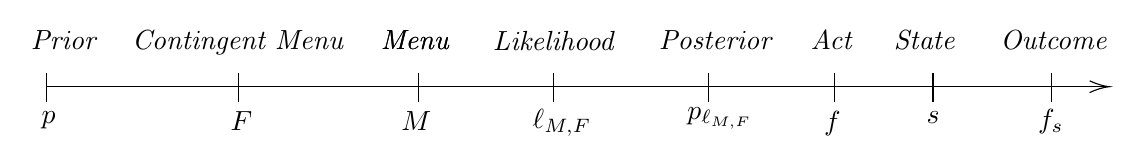
\begin{tikzpicture}[x=0.65pt,y=0.65pt,yscale=-1,xscale=1]
		% Uncomment if required: \path (0,472); % Set diagram left start at 0, and has height of 472

		% Draw the black horizontal line (arrow)
		\draw[opacity=1] (23,250) -- (614,250);

		% Draw the part of the horizontal arrow to the left of the vertical segment in black
		\draw[opacity=1] (23,250) -- (582,250);

		% Draw the part of the horizontal arrow to the right of the vertical segment in black
		\draw[opacity=1] (230,250) -- (614,250);

		% Draw the black oblique segments at the end of the horizontal arrow (pointing left)
		\draw[opacity=1, shift={(614,250)}, rotate=180]
		(10.93,-3.29) .. controls (6.95,-1.4) and (3.31,-0.3) .. (0,0) .. controls (3.31,0.3) and (6.95,1.4) .. (10.93,3.29);

		% Draw the small vertical segments below each word in black
		\draw[opacity=1] (23,242.5) -- (23,258.5);
		\draw[opacity=1] (130,242.5) -- (130,258.5);
		\draw[opacity=1] (230,242.5) -- (230,258.5);
		\draw[opacity=1] (305,242.5) -- (305,258.5);
		\draw[opacity=1] (391,242.5) -- (391,258.5);
		\draw[opacity=1] (461,242.5) -- (461,258.5);
		\draw[opacity=1] (516,242.5) -- (516,258.5);

		% The vertical segment below "Outcome, State, Act" in black
		\draw[opacity=1] (582,242.5) -- (582,258.5);
		\draw[opacity=1] (516,242.5) -- (516,258.5);
		\draw[opacity=1] (461,242.5) -- (461,258.5);

		% The words "Outcome, State, Act" in black
		\draw[opacity=1] (552,217.5) node [anchor=north west][inner sep=0.75pt] [align=left] {\textit{Outcome}};
		\draw[opacity=1] (492.74,217.5) node [anchor=north west][inner sep=0.75pt] [align=left] {\textit{State}};
		\draw[opacity=1] (446.45,217.5) node [anchor=north west][inner sep=0.75pt] [align=left] {\textit{Act}};

		% The vertical segment below "Menu" in black
		\draw[opacity=1] (230,242.5) -- (230,258.5);

		% The word "Menu" in black
		\draw[opacity=1] (207.58,217.5) node [anchor=north west][inner sep=0.75pt] [align=left] {\textit{Menu}};

		% The symbols "s, f_s, f" in black
		\draw[opacity=1] (511,262.15) node [anchor=north west][inner sep=0.75pt] {\(s\)};
		\draw[opacity=1] (573,261.15) node [anchor=north west][inner sep=0.75pt] {\(f_{s}\)};
		\draw[opacity=1] (454,262.15) node [anchor=north west][inner sep=0.75pt] {\(f\)};

		% The symbol "M" in black
		\draw[opacity=1] (219,262.15) node [anchor=north west][inner sep=0.75pt] {\(M\)};

		% Text for symbols (bottom) with black opacity
		\draw[opacity=1] (124,262.15) node [anchor=north west][inner sep=0.75pt] {\( F \)};
		\draw[opacity=1] (378,260.15) node [anchor=north west][inner sep=0.75pt] {\(p_{\ell_{M,F}}\)};
		\draw[opacity=1] (292,261.15) node [anchor=north west][inner sep=0.75pt] {\(\ell_{M,F}\)};
		\draw[opacity=1] (19,262.15) node [anchor=north west][inner sep=0.75pt] {\(p\)};

		% Text for labels (top) in black
		\draw[opacity=1] (69.29,217.5) node [anchor=north west][inner sep=0.75pt] [align=left] {\textit{Contingent Menu}};
		\draw[opacity=1] (207.58,217.5) node [anchor=north west][inner sep=0.75pt] [align=left] {\textit{Menu}};
		\draw[opacity=1] (362.16,217.5) node [anchor=north west][inner sep=0.75pt] [align=left] {\textit{Posterior}};
		\draw[opacity=1] (269.87,217.5) node [anchor=north west][inner sep=0.75pt] [align=left] {\textit{Likelihood}};
		\draw[opacity=1] (13,217.5) node [anchor=north west][inner sep=0.75pt] [align=left] {\textit{Prior}};
	\end{tikzpicture}

	\vspace{0.55cm}

	Expected utility of contingent menu \( F \) is

	\vfill
	\[
		\mathscr{U}(F)= \sum_{M} \sum_{s} p \left( s \right) F_{s} \left( M \right) \mathcal{U} \left(M ; \ell_{M, F} \right) .
	\] \pause

	\vfill

	The individual anticipates her choices and cost of temptation

	\vfill

	\[
		\begin{aligned}
			\mathcal{U} \left(M ; \ell_{M, F} \right) = & \max _{f \in M}\left\{\sum_{s} p_{\ell_{M, F}} \left( s \right) u \left( f_{s} ; \ell_{M, F} \right) + \alpha_{\ell_{M, F}} \sum_{s} p_{\ell^{*}_{M, F}} \left( s \right) u \left( f_{s} ; \ell^{*}_{M, F} \right) \right\}                                  \\
			                                            & -\max _{f^{\prime} \in M} \alpha _{\ell_{M, F}} \sum_{s} p_{\ell^{*}_{M, F}} \left( s \right) u\left(f^{\prime}_{s} ; \ell^{*}_{M, F} \right) . \: \: \: \text{\hyperlink{alpha}{\beamerbutton{Alpha?}}} \: \: \text{\hyperlink{cost}{\beamerbutton{Cost?}}}
		\end{aligned}
	\]

\end{frame}

\begin{frame}[noframenumbering]{Utility over contingent menus}

	Expected utility of contingent menu \( \textcolor{blue}{F} \) is

	\vfill
	\[
		\mathscr{U}(\textcolor{blue}{F})= \sum_{M} \sum_{s} p \left( s \right) F_{s} \left( M \right) \mathcal{U} \left(M ; \ell_{M, F} \right) .
	\]

	\vfill

	Only choices over \textcolor{blue}{contingent menus} are needed for identification.

	\vfill

	{\begingroup
		\transparent{0.2}

		\[
			\begin{aligned}
				\mathcal{U} \left(M ; \ell_{M, F} \right) = & \max _{f \in M}\left\{\sum_{s} p_{\ell_{M, F}} \left( s \right) u \left( f_{s} ; \ell_{M, F} \right) + \alpha_{\ell_{M, F}} \sum_{s} p_{\ell^{*}_{M, F}} \left( s \right) u \left( f_{s} ; \ell^{*}_{M, F} \right) \right\} \\
				                                            & -\max _{f^{\prime} \in M} \alpha _{\ell_{M, F}} \sum_{s} p_{\ell^{*}_{M, F}} \left( s \right) u\left(f^{\prime}_{s} ; \ell^{*}_{M, F} \right) .
			\end{aligned}
		\]
		\endgroup}

\end{frame}

\begin{frame}[noframenumbering]{Utility over contingent menus}

	{\begingroup
		\transparent{0.2}
		\[
			\mathscr{U}(\textcolor{blue}{F})= \sum_{M} \sum_{s} p \left( s \right) F_{s} \left( M \right) \mathcal{U} \left(M ; \ell_{M, F} \right) .
		\]

		\endgroup}

	Say the true likelihood \( \ell \) coincides with the distorted \( \textcolor{blue}{\ell^{*}} \):

	\vfill

	\[
		\begin{aligned}
			\mathcal{U} \left(M ; \textcolor{blue}{\ell^{*}} \right) = & \max _{f \in M}\left\{\sum_{s} p_{\textcolor{blue}{\ell^{*}}} \left( s \right) u \left( f_{s} ; \textcolor{blue}{\ell^{*}} \right) + \alpha_{\textcolor{blue}{\ell^{*}}} \sum_{s} p_{\textcolor{blue}{\ell^{*}}} \left( s \right) u \left( f_{s} ; \textcolor{blue}{\ell^{*}} \right) \right\} \\
			                                                           & -\max _{f^{\prime} \in M} \alpha _{\textcolor{blue}{\ell^{*}}} \sum_{s} p_{\textcolor{blue}{\ell^{*}}} \left( s \right) u\left(f^{\prime}_{s} ; \textcolor{blue}{\ell^{*}} \right) .
		\end{aligned}
	\]

	\vfill

	The second and third them cancel out, only EU under Bayesian updating remains.

	\vfill

	BDP \textbf{imply} non-Bayesian updating.

\end{frame}

\begin{frame}{Distorted likelihood}

	The distorted likelihood \( \ell^{*}_{S^{\prime}} \) at event \( S^{\prime} \) is the best one when any outcome is available:

	\vfill

	\[
		\ell^{*}_{S^{\prime}} \in \underset{\ell_{S^{\prime}}}{\arg \max} \: \max_{ x } \: u \left( x ; \ell_{S^{\prime}} \right) .
	\] \pause

	\vfill

	If a state has probability \( 0 \), its likelihood cannot be distorted. \pause

	\vfill

	\textbf{Asymmetric updating}: preferred likelihoods are not distorted.

\end{frame}

\begin{frame}{Main Axiom: Strategic Rationality for Best Likelihood}\label{srbl}

	\begin{axiom}\label{ax:srbl}
		There is no temptation when, all else equal, the available menu comprises the best choices from both the Bayesian update and the favourite posterior. \pause
	\end{axiom}

	\vfill

	\begin{table}[H]
		\centering
		\begin{minipage}{0.4\textwidth}
			\centering
			\begin{tabular}{c | c}
				\multicolumn{2}{c}{\textbf{Delegate}}                           \\
				State                & Menu                                     \\
				\hline
				{\color{blue}Good}   & \multirow{2}{*}{{\color{blue}\( w_p \)}} \\
				{\color{blue}Normal} &                                          \\
				Bad                  & \( w_q \)                                \\
			\end{tabular}
			\vspace{0.5cm} % Adjust vertical space between tables and caption
		\end{minipage}% Adjust the horizontal space between the tables and the symbol
		\begin{minipage}{0.4\textwidth}
			\centering
			\begin{tabular}{c | c}
				\multicolumn{2}{c}{}                                                 \\
				State                & Menu                                          \\
				\hline
				{\color{blue}Good}   & \multirow{2}{*}{{\color{blue}\( i_p, w_p \)}} \\
				{\color{blue}Normal} &                                               \\
				Bad                  & \( w_q \)                                     \\
			\end{tabular}
			\vspace{0.5cm} % Adjust vertical space between tables and caption
		\end{minipage} % Adjust the horizontal space between the tables and the symbol
		%\caption{Commitment under positive prior belief to avoid excessive investment.} % Add your caption here
		%\label{tab:commitment}
	\end{table}

	\begin{flushright}
		\hyperlink{srblapp}{\beamerbutton{Full}}
	\end{flushright}

\end{frame}

\begin{frame}[noframenumbering]{Main Axiom: Strategic Rationality for Best Likelihood}

	\begin{axiom}
		There is no temptation when, all else equal, the available menu comprises the best choices from both the Bayesian update and the favourite posterior.
	\end{axiom}

	\vfill

	\begin{table}[H]
		\centering
		\begin{minipage}{0.4\textwidth}
			\centering
			\begin{tabular}{c | c}
				\multicolumn{2}{c}{\textbf{Delegate}}                           \\
				State                & Menu                                     \\
				\hline
				{\color{blue}Good}   & \multirow{2}{*}{{\color{blue}\( w_p \)}} \\
				{\color{blue}Normal} &                                          \\
				Bad                  & \( w_q \)                                \\
			\end{tabular}
			\vspace{0.5cm} % Adjust vertical space between tables and caption
		\end{minipage}% Adjust the horizontal space between the tables and the symbol
		\( \succ \)
		\begin{minipage}{0.4\textwidth}
			\centering
			\begin{tabular}{c | c}
				\multicolumn{2}{c}{}                                                \\
				State                & Menu                                         \\
				\hline
				{\color{blue}Good}   & \multirow{2}{*}{{\color{blue}\(i_p, w_p \)}} \\
				{\color{blue}Normal} &                                              \\
				Bad                  & \( w_q \)                                    \\
			\end{tabular}
			\vspace{0.5cm} % Adjust vertical space between tables and caption
		\end{minipage} % Adjust the horizontal space between the tables and the symbol
		%\caption{Commitment under positive prior belief to avoid excessive investment.} % Add your caption here
		%\label{tab:commitment}
	\end{table}

	\begin{flushright}
		\hyperlink{srblapp}{\beamerbutton{Full}}
	\end{flushright}

\end{frame}

\begin{frame}[noframenumbering]{Main Axiom: Strategic Rationality for Best Likelihood}

	\begin{axiom}
		There is no temptation when, all else equal, the available menu comprises the best choices from both the Bayesian update and the favourite posterior.
	\end{axiom}

	\vfill

	\begin{table}[H]
		\centering
		\begin{minipage}{0.4\textwidth}
			\centering
			\begin{tabular}{c | c}
				\multicolumn{2}{c}{\textbf{Delegate}}                           \\
				State                & Menu                                     \\
				\hline
				{\color{blue}Good}   & \multirow{2}{*}{{\color{blue}\( w_p \)}} \\
				{\color{blue}Normal} &                                          \\
				Bad                  & \( w_q \)                                \\
			\end{tabular}
			\vspace{0.5cm} % Adjust vertical space between tables and caption
		\end{minipage}% Adjust the horizontal space between the tables and the symbol
		\begin{minipage}{0.4\textwidth}
			\centering
			\begin{tabular}{c | c}
				\multicolumn{2}{c}{}                                          \\
				State                & Menu                                   \\
				\hline
				{\color{blue}Good}   & \multirow{2}{*}{{\color{blue}\( 0 \)}} \\
				{\color{blue}Normal} &                                        \\
				Bad                  & \( w_q \)                              \\
			\end{tabular}
			\vspace{0.5cm} % Adjust vertical space between tables and caption
		\end{minipage} % Adjust the horizontal space between the tables and the symbol
		%\caption{Commitment under positive prior belief to avoid excessive investment.} % Add your caption here
		%\label{tab:commitment}
	\end{table}

	\begin{flushright}
		\hyperlink{srblapp}{\beamerbutton{Full}}
	\end{flushright}

\end{frame}

\begin{frame}[noframenumbering]{Main Axiom: Strategic Rationality for Best Likelihood}

	\begin{axiom}
		There is no temptation when, all else equal, the available menu comprises the best choices from both the Bayesian update and the favourite posterior.
	\end{axiom}

	\vfill

	\begin{table}[H]
		\centering
		\begin{minipage}{0.4\textwidth}
			\centering
			\begin{tabular}{c | c}
				\multicolumn{2}{c}{\textbf{Delegate}}                           \\
				State                & Menu                                     \\
				\hline
				{\color{blue}Good}   & \multirow{2}{*}{{\color{blue}\( w_p \)}} \\
				{\color{blue}Normal} &                                          \\
				Bad                  & \( w_q \)                                \\
			\end{tabular}
			\vspace{0.5cm} % Adjust vertical space between tables and caption
		\end{minipage}% Adjust the horizontal space between the tables and the symbol
		\( \sim \)
		\begin{minipage}{0.4\textwidth}
			\centering
			\begin{tabular}{c | c}
				\multicolumn{2}{c}{}                                          \\
				State                & Menu                                   \\
				\hline
				{\color{blue}Good}   & \multirow{2}{*}{{\color{blue}\( 0 \)}} \\
				{\color{blue}Normal} &                                        \\
				Bad                  & \( w_q \)                              \\
			\end{tabular}
			\vspace{0.5cm} % Adjust vertical space between tables and caption
		\end{minipage} % Adjust the horizontal space between the tables and the symbol
		%\caption{Commitment under positive prior belief to avoid excessive investment.} % Add your caption here
		%\label{tab:commitment}
	\end{table} \pause

	\vfill

	Under no BDP, all posteriors are "favourite" and the axiom implies no temptation.

	\vfill

	No temptation implies the model reduces to Expected utility and Bayesian updating.
\end{frame}

\begin{frame}{Main Result}\label{mainresult}

	\begin{theorem}
		Preferences over contingent menus are represented by equations \ref{eq:contmenu} and \ref{eq:menu} if and only if they satisfy \textbf{Strategic Rationality for Best Likelihood} and other regularity axioms.
	\end{theorem}

	\vfill

	\begin{equation}\label{eq:contmenu}
		\mathscr{U}(F)= \sum_{M} \sum_{s} p \left( s \right) F_{s} \left( M \right) \mathcal{U} \left(M ; \ell_{M, F} \right) .
	\end{equation}

	\vfill

	\begin{equation}\label{eq:menu}
		\begin{aligned}
			\mathcal{U} \left(M ; \ell_{M, F} \right) = & \max _{f \in M}\left\{\sum_{s} p_{\ell_{M, F}} \left( s \right) u \left( f_{s} ; \ell_{M, F} \right) + \alpha_{\ell_{M, F}} \sum_{s} p_{\ell^{*}_{M, F}} \left( s \right) u \left( f_{s} ; \ell^{*}_{M, F} \right) \right\} \\
			                                            & -\max _{f^{\prime} \in M} \alpha _{\ell_{M, F}} \sum_{s} p_{\ell^{*}_{M, F}} \left( s \right) u\left(f^{\prime}_{s} ; \ell^{*}_{M, F} \right) \:
		\end{aligned}
	\end{equation}

	\vfill

	Prior belief \( p \), utilities \( u \), distorted likelihoods \( \ell^{*} \) and weights \( \alpha \) are "unique". \hyperlink{axiomsb1main}{\beamerbutton{Axioms?}}

\end{frame}

\begin{frame}{Why this model: observability and identification}
	The primitive objects of choice, contingent menus, are observable, contrary to

	\vfill

	\begin{wideitemize}
		\item Choice of beliefs \citep{brunnermeierOptimalExpectations2005,koszegiUtilityAnticipationPersonal2010};
		\item Choice of probability to forget \citep{benabou2016mindful}.
	\end{wideitemize}

	\vfill

	Choices of information sources do not allow identification \citep{eliazCanAnticipatoryFeelings2006}.

	\vfill

	These papers only provide "if" results, hard to distinguish from other theories.
\end{frame}

\begin{frame}{Why this model: multiple selves and updating}
	Individual as the unit of choice, multiple selves render welfare analysis hard.

	\vfill

	Under multiple selves, choices are dynamically inconsistent.

	\vfill

	BDP and non-Bayesian updating are not disjoint, the first implies the second.
\end{frame}


\begin{frame}{Conclusion}
	Theory of BDP and belief updating tested via choices of contingent menus.

	\vfill

	Dynamically consistent individual anticipates she distorts beliefs to satisfy her BDP.

	\vfill

	Asymmetric updating and no distortion of zero probability events.

	\vfill

	Identification of BDP, non-Bayesian updating and strength of motivated reasoning.

	\vfill

	Other applications in the paper:

	\vfill

	\begin{wideitemize}
		\item donors avoid and distort information about their impact;
		\item politicians send poor information to induce polarisation.
	\end{wideitemize}

\end{frame}

\begin{frame}[noframenumbering,plain]

	\frametitle{References}

	%\nocite{*}
	\bibliography{Others/bib}
	\bibliographystyle{apacite}


\end{frame}

\appendix

\begin{frame}[noframenumbering,plain]{Cost of self-control}\label{alpha}

	Identification of \( \alpha_{\ell} \) allows elaborating on its behavioural meaning

	\vfill

	\[
		\alpha_{\ell} = \frac{\mathcal{U} \left( \left\{f, x \right\}, \ell \right) - \mathcal{U} \left( \left\{f, x^{\prime} \right\}, \ell \right) }{u \left( x , \ell \right) - u \left( x^{\prime} , \ell \right)} .
	\]

	\vfill

	It is the marginal cost of self-control at likelihood \( \ell \). \hyperlink{fullmodel}{\beamerbutton{Back}}

\end{frame}

\begin{frame}[noframenumbering,plain]{Alternative representation with cost}\label{cost}

	The representation can be written as either

	\[
		\begin{aligned}
			\mathcal{U} \left(M ; \ell_{M, F} \right) = & \max _{f \in M}\left\{\sum_{s} p_{\ell_{M, F}} \left( s \right) u \left( f_{s} ; \ell_{M, F} \right) +\alpha _{\ell_{M, F}} \sum_{s} p_{\ell^{*}_{S_{M, F}}} \left( s \right) u \left( f_{s} ; \ell^{*}_{S_{M, F}} \right) \right\} \\
			                                            & -\max _{f^{\prime} \in M} \alpha _{\ell_{M, F}} \sum_{s} p_{\ell^{*}_{S_{M, F}}} \left( s \right) u\left(f^{\prime}_{s} ; \ell^{*}_{S_{M, F}} \right) ,
		\end{aligned}
	\]

	or

	\[
		\mathcal{U} \left(M ; \ell_{M, F} \right) = \max _{f \in M}\left\{\sum_{s} p_{\ell_{M, F}} \left( s \right) u \left( f_{s} ; \ell_{M, F} \right) - \alpha_{\ell_{M, F}} c \left( f, u, S_{M,F} \right) \right\} .
	\]

	\begin{flushright}
		\hyperlink{fullmodel}{\beamerbutton{Back}}
	\end{flushright}

\end{frame}

\begin{frame}[noframenumbering,plain]{Axioms: Basics}\label{axiomsb1main}

	\begin{axiom}\label{ax:order}
		\labelname{axn:order}{Order and Continuity} (\textbf{Order}). Preferences over contingent menus are a continuous weak order. \hyperlink{axiomsb1}{\beamerbutton{Full}}
	\end{axiom}

	\begin{axiom}\label{ax:degeneracy}
		\labelname{axn:degeneracy}{Nondegeneracy}

		(\textbf{Nondegeneracy}). There exist at least one outcome better than another. \hyperlink{axiomsb2}{\beamerbutton{Full}}

	\end{axiom}

	\begin{axiom}\label{ax:sindependence}
		\labelname{axn:sindependence}{State Independence}

		(\textbf{\textbf{State Independence}}). Preferences over outcomes do not depend on the state.
	\end{axiom}

	\begin{axiom}\label{ax:support}
		\labelname{axn:support}{Full Support}

		(\textbf{\textbf{Full support}}). The individual assigns ex-ante positive probability to all states.
	\end{axiom}

	\begin{flushright}
		\hyperlink{mainresult}{\beamerbutton{Back}}
	\end{flushright}

\end{frame}

\begin{frame}[noframenumbering,plain]{Axioms: Identical Inference Independence}\label{independence}

	\begin{axiom}\label{ax:independence}
		The individual is only indifferent between mixtures of contingent menus inducing the same inference.
	\end{axiom}

	\vfill

	\begin{table}[H]
		\centering
		\begin{minipage}{0.4\textwidth}
			\centering
			\begin{tabular}{c | c}
				\multicolumn{2}{c}{\textbf{Delegate}}                              \\
				State                & Menu                                        \\
				\hline
				{\color{blue}Good}   & \multirow{2}{*}{{\color{blue}\( i_p, n \)}} \\
				{\color{blue}Normal} &                                             \\
				Bad                  & \( n \)                                     \\
			\end{tabular}
			\vspace{0.5cm} % Adjust vertical space between tables and caption
		\end{minipage}% Adjust the horizontal space between the tables and the symbol
		\begin{minipage}{0.4\textwidth}
			\centering
			\begin{tabular}{c | c}
				\multicolumn{2}{c}{}                                             \\
				State                & Menu                                      \\
				\hline
				{\color{blue}Good}   & \multirow{2}{*}{{\color{blue}\( n, w \)}} \\
				{\color{blue}Normal} &                                           \\
				Bad                  & \( n \)                                   \\
			\end{tabular}
			\vspace{0.5cm} % Adjust vertical space between tables and caption
		\end{minipage} % Adjust the horizontal space between the tables and the symbol
		%\caption{Commitment under positive prior belief to avoid excessive investment.} % Add your caption here
		%\label{tab:commitment}
	\end{table}

	\begin{flushright}
		\hyperlink{independenceapp}{\beamerbutton{Full}}
	\end{flushright}

\end{frame}

\begin{frame}[noframenumbering,plain]{Axioms: Set-Betweenness}\label{betweenness}

	\begin{axiom}\label{ax:sbetweenness}
		The individual is weakly worse if a menu is enhanced with ex-ante dominated options, because these induce temptation.
	\end{axiom}

	\vfill

	\begin{table}[H]
		\centering
		\begin{minipage}{0.4\textwidth}
			\centering
			\begin{tabular}{c | c}
				\multicolumn{2}{c}{\textbf{Delegate}}                         \\
				State                & Menu                                   \\
				\hline
				{\color{blue}Good}   & \multirow{2}{*}{{\color{blue}\( n \)}} \\
				{\color{blue}Normal} &                                        \\
				Bad                  & \( n \)                                \\
			\end{tabular}
			\vspace{0.5cm} % Adjust vertical space between tables and caption
		\end{minipage}% Adjust the horizontal space between the tables and the symbol
		\( \succ \)
		\begin{minipage}{0.4\textwidth}
			\centering
			\begin{tabular}{c | c}
				\multicolumn{2}{c}{}                                              \\
				State                & Menu                                       \\
				\hline
				{\color{blue}Good}   & \multirow{2}{*}{{\color{blue}\(i_p, n \)}} \\
				{\color{blue}Normal} &                                            \\
				Bad                  & \( n \)                                    \\
			\end{tabular}
			\vspace{0.5cm} % Adjust vertical space between tables and caption
		\end{minipage} % Adjust the horizontal space between the tables and the symbol
		%\caption{Commitment under positive prior belief to avoid excessive investment.} % Add your caption here
		%\label{tab:commitment}
	\end{table}

	\begin{flushright}
		\hyperlink{betweennessapp}{\beamerbutton{Full}}
	\end{flushright}


\end{frame}

\begin{frame}[noframenumbering,plain]{Axioms: Basics I}

	\begin{axiom}\label{ax:orderapp}
		\labelname{axn:orderapp}{Order} (\textbf{Order}). The ranking \(\succsim\) is complete and transitive.

	\end{axiom}

	\vfill

	\begin{axiom}\label{ax:continuityapp}\label{axiomsb1}
		\labelname{axn:continuityapp}{Continuity}

		(\textbf{Continuity}). For all contingent menus \( F \) the sets

		\[
			\left\{ F^{\prime} \mid F^{\prime} \succsim F \right\} \: and \: \left\{ F^{\prime} \mid F^{\prime} \precsim F \right\}
		\]

		are closed.

	\end{axiom}

	\begin{flushright}
		\hyperlink{axiomsb1main}{\beamerbutton{Back}}
	\end{flushright}

\end{frame}

\begin{frame}[noframenumbering,plain]{Axioms: Basics II}\label{axiomsb2}

	\begin{axiom}\label{ax:degeneracyapp}
		\labelname{axn:degeneracyapp}{Nondegeneracy}

		(\textbf{Nondegeneracy}). There exist outcomes \(y, y^{\prime}\) in \(X\) for which \(y \succ y^{\prime}\).

	\end{axiom}

	\vfill

	\begin{axiom}\label{ax:sindependenceapp}
		\labelname{axn:sindependenceapp}{State Independence}

		(\textbf{\textbf{State Independence}}). For all contingent menus \( F \), menus \( L, L^{\prime}, M \) and states \( s, s^{\prime} \),

		\[
			F \succsim F_{L s M \rightarrow L^{\prime} s M} \: \Rightarrow \: F \succsim F_{L s^{\prime} M \rightarrow L^{\prime} s^{\prime} M} .
		\]

	\end{axiom}


	\vfill

	\begin{axiom}\label{ax:appsupport}
		\labelname{axn:appsupport}{Full Support}

		(\textbf{\textbf{Full Support}}). For each state \(s\), there exist contingent menus \(F \) and \(F^{\prime}\) such that for all menus \( M \) it holds that \(F_{s^{\prime}} \left( M \right) =F^{\prime}_{s^{\prime}} \left( M \right)\) for every \(s^{\prime} \neq s \) and \(F \nsim F^{\prime}\).

	\end{axiom}

	\begin{flushright}
		\hyperlink{axiomsb1main}{\beamerbutton{Back}}
	\end{flushright}
\end{frame}

\begin{frame}[noframenumbering,plain]{Axioms: Identical Inference Independence}

	The support of \( F \) is

	\[ \mathcal{M}_{F} := \left\{ M \in \mathcal{M} \: \mid \: F_{s} \left( M \right) > 0 \: \text{for some} \: s \in S \right\} . \]

	\begin{definition}\label{def:ii}
		\labelname{def:ii}{II}

		(\textbf{Identical Inference (II)})
		Two contingent menus \(F\) and \(F^{\prime}\) satisfy \textbf{identical inference} if, for each menu \(M \in \mathcal{M}_{F} \cap \mathcal{M}_{F^{\prime}}\) their likelihood is the same \(\ell_{M, F} = \ell_{M, F^{\prime}} \).

	\end{definition}

	\begin{axiom}\label{ax:independenceapp}\label{independenceapp}
		\labelname{axn:independenceapp}{II Independence}

		(\textbf{II Independence}). For all \(0<\lambda \leq 1\) and contingent menus \(F, F^{\prime}, F^{\prime \prime} \) such that \(F\) and \(F^{\prime \prime}\) satisfy \usename{def:ii} and \(F^{\prime}\) and \(F^{\prime \prime}\) satisfy \usename{def:ii}, \(F \succsim F^{\prime}\) if and only if \(\lambda F+ \left( 1-\lambda \right) F^{\prime \prime} \succsim \lambda F^{\prime} + \left( 1-\lambda \right) F^{\prime \prime}\).
	\end{axiom}

	\begin{flushright}
		\begin{flushright}
			\hyperlink{independence}{\beamerbutton{Back}}
		\end{flushright}
	\end{flushright}

\end{frame}

\begin{frame}[noframenumbering,plain]{Axioms: Set-Betweenness}\label{betweennessapp}

	Substitute from \( F \) any occurrence of \( M \) with \( M^{\prime} \) to get \( F_{M \rightarrow M^{\prime}} \).

	\vfill

	\begin{axiom}\label{ax:betweennessapp}
		\labelname{axn:betweennessapp}{Set-Betweenness}

		(\textbf{Set-Betweenness}). For all contingent menus \( F \) and menus \( M, M^{\prime} \),

		\vfill

		\[
			F  \succsim F_{M \rightarrow M^{\prime}} \Rightarrow F  \succsim F_{M \rightarrow M \cup M^{\prime}} \succsim F_{M \rightarrow M^{\prime}} .
		\]

	\end{axiom}

	\begin{flushright}
		\hyperlink{betweenness}{\beamerbutton{Back}}
	\end{flushright}

\end{frame}

\begin{frame}[noframenumbering,plain]{Axioms: Strategic Rationality for Best Likelihood}\label{srblapp}

	Substitute from \( F \) any occurrence of \( M \) with \( M^{\prime} \) to get \( F_{M \rightarrow M^{\prime}} \).

	\vfill

	For each menu \( M \) and likelihood \( \ell \) define the set

	\[
		M_{\ell} := \left\{ f \in M \: \mid \: F \succsim F_{\left\{ f \right\} \rightarrow \left\{ f^{\prime} \right\}} \: \text{for all} \: f^{\prime} \in M \: \text{and} \: F \: \text{such that} \: \ell_{\left\{f \right\}, F} = \ell \right\} .
	\]

	\begin{axiom}\label{ax:appsrbl}
		\labelname{axn:appsrbl}{SRBL}

		(\textbf{Strategic Rationality for Best Likelihood}). For all contingent menus \( F \), menus \( M, M^{\prime} \), events \( E \) and likelihoods \( \ell_E \), if \( \left( M \cup M^{\prime} \right)_{\ell_E} \cap \left( M \cup M^{\prime} \right)_{\ell^{*}_{E}} \neq \emptyset \) for some \( \ell_{E}^{*} \), then

		\[
			F \succsim F_{M \rightarrow M^{\prime}} \Rightarrow F \sim F_{M \rightarrow M \cup M^{\prime}} .
		\]

	\end{axiom}

	\begin{flushright}
		\hyperlink{srbl}{\beamerbutton{Back}}
	\end{flushright}


\end{frame}

\end{document}